\chapter{Evaluation} \label{chap:evaluation}

The methods of evaluating the performance of classifiers in LOS prediction
that are discussed in the literature encompass a wide range of medical
domains and learning problems, which presents us with a challenge when we
decide how to evaluate our work. Here we have chosen to rigorously evaluate
our results (such as using stratified cross-validation when others may have
used a single training-test split), while still using performance measures
comparable to the literature and suitable for our particular learning problem.
This chapter discusses the data sets, procedure and performance measures used
in evaluating our work.

\section{Data Sets}
In our work we obtained two independent sets of LOS data, one specifically for
trauma and the other a general, hospital-wide set.

\subsection{Trauma LOS Data}
\subsubsection{Collection}
The data set used consisted of trauma registry data from the trauma centre
at the Royal Prince Alfred Hospital, a major trauma centre in New South Wales,
Australia. It covered all adult (age 15 and over) inpatient admissions to the
trauma centre from 2007--2011. 

All patients were first admitted to the trauma ward until discharged
or transferred to an appropriate unit within the hospital. A single trained
data manager recorded a variety of attributes about the admitted patient,
such as age, gender, blood pressure, mechanism of injury and body regions
that were injured. We received this data in a Microsoft Excel spreadsheet.

\subsubsection{Characteristics}
There were 2546 patient records in the data set we received, comprising of 79
features, one of which was the target variable \texttt{los48}.
\texttt{los48} was a binary variable -- that is, it could only take two
values, 0 or 1 -- with 1 indicating that the patient stayed two days or less,
and 0 indicating a stay of greater than 2 days.

\subsection{General Hospital LOS Data}
By collaborating with our colleagues from the University of Minho in Portugal,
we were able to obtain LOS data for all inpatient hospitalisations from
2000--2013 at the Hospital das Foras Armadas in Lisboa, Portugal. The data
contained 26462 inpatient records spanning all medical departments within the
hospital, comprising 15 features that were not specific to any medical domain.

\section{Evaluation Procedure}
\subsection{Steps Involved}
The steps that we took to evaluate the performance of the various classifiers
and feature selection methods were:
\begin{enumerate}
\item The trauma LOS data was cleaned and preprocessed as described in Chapter
\ref{chap:preprocess}, giving us two data sets: one with and one without
discretisation. The general LOS data from Portugal was already cleaned when we
received it; however, we discretised the continuous \texttt{los} variable to
the same categories as for the trauma data (2 days or less, greater than 2
days), normalised the numeric attribute \texttt{prev\_admissions}, and derived
both a discretised and non-discretised data set. This resulted in 4 sets of
data.
\item For each data set, we evaluated the effect of the 4 automatic feature
selection methods on each of the 8 classifiers described in Chapter
\ref{chap:classification}, giving us 32 configurations for each data set, over
4 sets. Evaluation was performed using \textit{ten-fold stratified
cross-validation} (described below).
\item For the two trauma LOS data sets, we additionally evaluated the two
manual feature selection methods with all 8 classifiers. Recall from Section
\ref{sec:manual} that one of the feature sets is from the key previous work
on trauma LOS prediction that we use as a baseline, and the other feature set
is a set of features included through consultation with a domain expert.
\end{enumerate}

\subsection{Ten-fold Stratified Cross-Validation}
Cross-validation is a method of evaluating the performance of a learning
algorithm. The entire data set is partitioned into $k$ subsets, and the
learning algorithm is trained on $k-1$ of these subsets and tested on one. This
is repeated $k$ times, so that each of the subsets is used exactly once as a
test set. After each iteration of training and testing, called a \textit{fold},
various performance measures about the classifier are recorded. At the end of
the $k$ folds, the $k$ performance measures obtained are averaged to arrive at
a final measure of performance. \textit{Stratified} cross-validation ensures
that the proportion of each class in each of the $k$ subsets is approximately
the same as in the entire data set. This reduces the effect of random uneven
class representation in the partitioned $k$ subsets during the cross-validation
process.

We use $k=10$ folds for our stratified cross-validation, which has been
considered the standard method of measuring the performance of a learning
algorithm on a given data set \cite{Witten2005}.

\subsection{Technical Details}
Here we specify the technical details of our work: namely, the programming
languages and software used in our entire procedure.

\subsubsection{Repository}
All code relating to this work, including the \LaTeX\ code for this document,
as well as results from our evaluations are available publicly online at
\url{https://github.com/tianyupu/hons-thesis}. However, we were not able to
obtain permission from neither the Royal Prince Alfred Hospital nor the
Hospital das Foras Armadas to make the data publicly available due to the
privacy of patient information. Interested readers should discuss with the
author.

\subsubsection{Software Used}
For initial exploration and cleaning of data, we used Microsoft Excel 2007
as the data was already in spreadsheet format. This was then exported to
CSV. For the conversion to ARFF, and evaluation of the automatic
feature selection methods and classification algorithms, we used the latest
developer version of WEKA, 3.7.11 \cite{Hall2009}. We used WEKA exclusively
through the command-line interface so that we could automate and configure
our experiments easily using scripts which we wrote (see Section
\ref{sec:code}).

\subsubsection{Code Written}
\label{sec:code}
\todo{attach code in appendix?}
Leading and trailing whitespace was removed and feature names transformed using
code written in Python to manipulate the CSV. All runs of WEKA were executed by
a program we wrote in Bash (a Unix shell) script. This program was able to run
WEKA with the following features:
\begin{itemize}
\item The ability to specify filenames corresponding to the input training data
and the specification of classification or feature selection algorithms to run
\item ROC curve data output can be optionally enabled and saved to disk after
each cross-validation pass
\item An experiment can be repeated an arbitrary number of times -- this is
specified by the user upon invoking the script (default is one time)
\item The ability to specify the inclusion of a random number seed -- this is
necessary for repetitions of runs to generate different cross-validation splits
\item Model information and performance measures are saved to disk after each
cross-validation
\end{itemize}

Because of the large numbers of results we obtained, we also wrote scripts in
Bash and Python to process and summarise the performance measures we required.
If we ran a set of classifiers 50 times in an experiment, the script would
retrieve all 50 outputs of a performance measure (such as accuracy, described
in the next section) for each classifier, and compute the mean and confidence
interval (also discussed in the next section) in a single output that we could
then save as CSV.

In order to implement our novel Ranked Distance function (Section
\ref{sec:rankeddist}), we created our own class within the WEKA Java package
hierarchy. This was implemented in Java and needed to implement the correct
interfaces and override the right inherited methods in order for the $k$-NN
classifier in WEKA to be able to use it as a distance function. This also
involved updating certain properties of the \texttt{weka.jar} executable in
order to use the new class, as well as building the entire WEKA source. The
development environment we used was Eclipse \todo{insert version}, and the
source was built using the 1.7 Java runtime. \todo{double check}

\section{Performance Measures}
There are many ways to evaluate the performance of learning algorithms. The
two measures we will use are the \textit{accuracy} and the \textit{area under
the receiver operating characteristic (ROC) curve}, commonly abbreviated AUC.

\subsection{Accuracy}
The accuracy is a common measure of performance for classification algorithms,
and indicates the proportion of examples that were classified correctly from
a given data set. Mathematically, assuming a two-class scenario, the expression
is:
\begin{equation*}
\mathrm{Accuracy} = \dfrac{TP + TN}{TP + TN + FP + FN}
\end{equation*}
where:
\begin{itemize}
  \item $TP$ is the number of \textit{true positives} -- that is, the number of
  examples belonging to class 1 that were classified as belonging in class 1;
  \item $TN$ is the number of \textit{true negatives}, which is the number of
  examples belonging to class 0 that were classified as belonging to class 0;
  \item $FP$ is the number of \textit{false positives}, which is the number of
  examples that should have been classified 0 but were classified as 1; and
  \item $FN$ is the number of \textit{false negatives}, which is the number of
  examples that should have been classified 1 but were classified as 0.
\end{itemize}

The accuracy can also be expressed more simply and intuitively as
the number of correct classifications out of the total number of examples,
but the terms introduced above will be necessary to understand the
AUC measure below.

We use accuracy as a performance measure as it is often used in previous work,
which allows us to compare our work with others. Accuracy is also relatively
straightforward to understand and interpret.

\subsection{Area Under the Curve}
The area under the receiver operating characteristic (ROC) curve, often
abbreviated AUC, is a measure of the ability of a binary classifier to
distinguish between members of the two classes. Let the \textit{true
positive rate} be $\dfrac{TP}{TP + FN}$ and the \textit{false positive rate}
be $\dfrac{FP}{FP + TN}$. The ROC curve is a plot of the true positive rate
on the vertical axis against the false positive rate on the horizontal axis.
The area under this curve will lie between 0 and 1, with 1 indicating a
100\% true positive rate and 0\% false positives (that is, everything was
classified correctly). The AUC of randomly picking between the two classes
with equal probability is 0.5, with a ROC curve that is a straight line
dividing the graph diagonally in half. Figure \ref{fig:sampleroc} shows
two ROC curves on the same graph:

\begin{figure}[h]
\centering
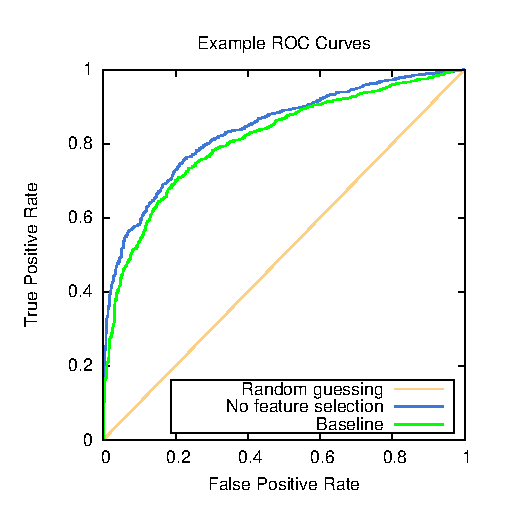
\includegraphics{images/method/example-roc.eps}
\caption{Two ROC curves on the same graph. Note that the straight line from
the bottom left corner to the top right corner indicates an AUC of 0.5. Curves
which head towards the top left corner indicate increasing AUC.}
\label{fig:sampleroc}
\end{figure}

The AUC has not been commonly used in the literature to evaluate LOS
classification problems, but we have included it in our work for a number of
reasons. Firstly, it measures an aspect of classifiers that accuracy does not,
and which is more important and useful in the domain: the ability to
discriminate between instances of two classes. Recall from Chapter
\ref{chap:classification} that 0R will always predict the majority class --
this means that it will be evaluated positively on the basis of accuracy
as long as there are sufficiently more examples of one class than the other.
However, the AUC of the classifier will be \textit{less} than 0.5, because it
is less able to distinguish between the two classes than random guessing is,
due to the fact that it only ever predicts unseen examples to be in the
majority class. Secondly, previous work on trauma LOS prediction by Dinh et al.
also used the AUC as the key measure by which they evaluated their model
\cite{Dinh2013a}, and we would like our work to be comparable to theirs.

\subsection{Confidence Intervals}
In order to compare our results with our baseline, the work of Dinh et. al.
\citep{Dinh2013a}, as well as quantify the level of confidence we have in
our performance measures, we constructed 95\% confidence intervals for the
mean accuracy and AUC.

For each classifier, let the population of all of its accuracy (or AUC)
scores be some random variable $X$, which follows a distribution whose
parameters (such as mean and standard deviation) we do not know.
The Central Limit Theorem from statistics states that given a random
sample of $n$ items from $X$, namely $X_1,X_2,\dots,X_n$, the sample mean
$\bar{x}$
is approximately normally distributed when $n$ is at least roughly around 30
and the $X_i$'s are independent and identically distributed \cite{Phipps2001}.

Consequently, we can construct a $(1-\alpha)$\% normal confidence interval for
$\bar{x}$ -- where $\alpha$ is commonly called the
\textit{significance level} -- as follows \cite{Wasserman2003}:
\begin{equation*}
  \left[\bar{x} - z_{1-\alpha/2}\dfrac{s}{\sqrt{n}},
    \bar{x} + z_{1-\alpha/2}\dfrac{s}{\sqrt{n}}\right]
\end{equation*}
where $\bar{x}$ is the sample mean, $\alpha$ is the significance level
(5\% or $0.05$ in our case), $s$ is the sample standard deviation, $n$
is the number of observations in our sample, and $z_{1-\alpha/2}$ is the value
of the standard normal variable $Z \sim \mathcal{N}(0,1)$ with cumulative
probability $1-\alpha/2$.

These confidence intervals can be constructed 

In our work, we repeated the ten-fold stratified cross-validation procedure
ten times, leading to $n=100$ samples with which to obtain our confidence
estimates.

\subsection{Tests for Statistical Significance}
To decide whether or not the difference in values of each measure between
classifiers and feature selection methods was statistically significant,
paired $t$-tests at a significance level of 0.05 were conducted.
\todo{elaborate}

\section{Summary}
In this section we described our method of evaluating the performance of each
classifier and feature selection method that we use. We used accuracy and the
area under the curve to measure two different aspects of our classifiers, and
we obtained these figures using stratified ten-fold cross-validation. Paired
$t$-tests were conducted to test for statistical significance.
